La versione attuale dell'UR5 \'{e} quella appartenente alla \textbf{e-series}, rilasciata nel 2018. 
Tuttavia, in questa tesi, viene utilizzata la versione precedente della famiglia \textbf{CB3}, commercializzata a partire dal 
2008.
\begin{figure}[H]
    \centering
    \includegraphics*[width=0.5\textwidth]{images/ur5.png}
    \caption{UR5/CB3}
    \label{fig:ur5}
\end{figure}
All'estremit\'{a} del robot \'{e} possibile installare un \textbf{end effector}, ossia un dispositivo concepito 
per la manipolazione degli oggetti che fornisce l'unica possibile interazione con l'ambiente esterno.
Il carico massimo sopportabile dall'UR5 dipende dall'offset del centro di gravit\'{a}, ossia la distanza tra l'estremit\'{a}  
del braccio robotico (punto di applicazione dell'end effector) e il centro di gravit\'{a} dell'UR5. 
\begin{figure}[H]
    \centering
    \includegraphics*[width=0.7\textwidth]{images/payload.png}
    \caption{Andamento del carico massimo sopportabile rispetto all'offset del centro di gravit\'{a}}
    \label{fig:payload}
\end{figure}
Come si pu\'{o} notare in Figura \ref{fig:payload}, l'UR5 \'{e} in grado di sopportare un carico massimo di 5 Kg finch\'{e} 
l'estensione del braccio non supera i 350mm. Da qui in poi al crescere dell'offset seguir\'{a} una diminuzione del carico massimo 
applicabile.
L'UR5 \'{e} collegato ad una \textbf{control box} che \'{e} un dispositivo alimentato elettricamente 
in grado di fornire energia sia al robot che alle periferiche collegate ad esso. Sulla control box \'{e} presente poi un'uscita 
ethernet per la connessione ad un PC per il controllo remoto, da cui vengono lanciati tutti 
gli applicativi sviluppati.
\begin{figure}[H]
    \centering
    \begin{subfigure}[b]{0.4\textwidth}
        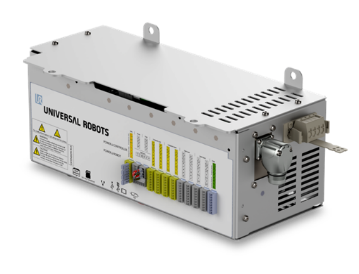
\includegraphics[width=\textwidth]{images/control-box.png}
        \caption{Control box}
        \label{fig:control-box}
    \end{subfigure}
    ~ %add desired spacing between images, e. g. ~, \quad, \qquad, \hfill etc. 
      %(or a blank line to force the subfigure onto a new line)
    \begin{subfigure}[b]{0.4\textwidth}
        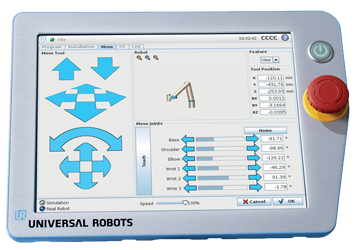
\includegraphics[width=\textwidth]{images/teach_pendant.png}
        \caption{Teach pendant}
        \label{fig:teach_pendant}
    \end{subfigure}
    \caption{}
    \label{fig:box-pendant}
\end{figure}
In Figura \ref{fig:box-pendant} vengono mostrati la control box e il \textbf{Teach Pendant}, un dispositivo touchscreen collegato 
alla control box che consente il controllo diretto del robot. Sul Teach Pendant \'{e} eseguita un'interfaccia chiamata \textbf{Polyscope} 
che permette la programmazione dei movimenti del robot e il cambiamento di alcune sue impostazioni. 
Per poter controllare l'UR5 tramite ROS \'{e}, tuttavia, necessario installare sul Teach Pendant il plugin \textbf{externalcontrol.urcap}, 
creare un nuovo programma su Polyscope che preveda l'utilizzo del plugin ed impostare l'indirizzo IP del computer remoto da cui 
verranno lanciati i nodi ROS.
